\chapter{Current state of Kdyby}

To be able to lay out the roadmap, first we have to know the current state of each Kdyby package, the original purpose and the current requirements. We will only review those packages that actually made it to production and at least one usable version was released.

I have created few GitHub repositories as a reminder for me to start working on some other web application development problems. I did start to work on some of them, for example on DoctrineForms, but it was never "officially released". We will not discuss these incomplete packages in this thesis.

\section{State of the project}

The most relevant problem is the compatibility with new versions of the libraries, that Kdyby integrates. Current version of \gls{nette} is 2.4 and the 3.0 is being developed, but some of Kdyby packages support only \gls{nette} 2.2 or older.

The other problems appear only when you interact with the source code which is still really important for me as a maintainer and for the contributors. Also good maintainable code attracts more programmers to use it and contribute. But, there is no coding standard being enforced automatically on any package and no static analysis tool is checking the code. On the other hand almost all of the packages have unit and integration tests and linter checking the code for multiple versions of PHP.

\begin{figure} \label{fig:php:supported-versions}
  \centering
    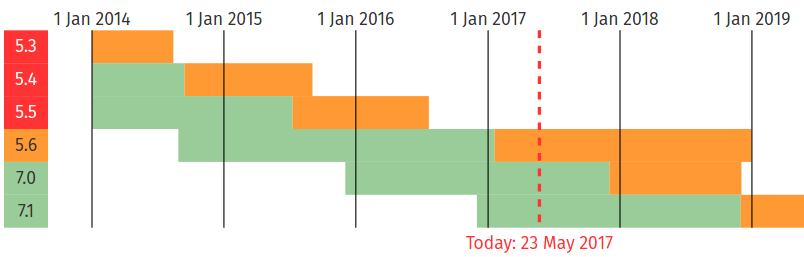
\includegraphics[width=1\textwidth]{src/assets/php-supported-versions.png}
  \caption{Supported PHP Versions. Green is active support, orange is security fixes only. Up-to-date version is at \url{http://php.net/supported-versions.php}}
\end{figure}
Most of the packages are compatible with PHP 5.4, but \fnurl{PHP 5.4 had end of life at \printdate{2015-09-03}}{http://php.net/eol.php} and is no longer supported by PHP developers.

The PHP 5.5 had end of life at \printdate{2016-06-21} and PHP 5.6 is currently in the phase of security fixes only and will have end of life at \printdate{2018-12-31}. As you can see on the graph~\ref{fig:php:supported-versions}, everyone should be migrating to PHP 7.0 by now. But the developer has to consider what PHP versions the libraries support, upgrade them first and then migrate the application.

\section{State of each package}

This section reviews each package separately, considers the original purpose and sums up the current state.

\hiddensubsection{Doctrine} \label{sec:state:doctrine}

\gls{kDoctrine} is an integration of \gls{doctrine} into Nette Framework. But it has cumulated a lot of responsibilities, that don't belong to it

\gls{doctrine} itself is separated into several packages, mainly \fnurl{doctrine/orm}{https://github.com/doctrine/doctrine2}, \fnurl{doctrine/common}{https://github.com/doctrine/common}, \fnurl{doctrine/annotations}{https://github.com/doctrine/annotations}, \fnurl{doctrine/cache}{https://github.com/doctrine/cache} and \fnurl{doctrine/collections}{https://github.com/doctrine/collections}. What started as a monolith integration in Kdyby, got separated into \gls{kEvents}~\ref{sec:state:events}, \gls{kConsole}~\ref{sec:state:console}, \gls{kAnnotations}~\ref{sec:state:annotations} and \gls{kDoctrineCache}~\ref{sec:state:doctrine-cache} for reusability.

I have already started extracting few of them in the past, for example an entity prototyping tool~\ref{sec:state:doctrine-magic-accessors}, collection utilities~\ref{sec:state:doctrine-collections-lazy}, \ref{sec:state:doctrine-collections-readonly} and helper for loading big SQL scripts to the database~\ref{sec:state:doctrine-dbal-batch-import}.

There is a big issue \fnurl{Chop up the package}{https://github.com/Kdyby/Doctrine/issues/238} that discusses what other parts should be separated and dropped completely.

New versions of Nette and \gls{doctrine} were released and completely new versions are being prepared, which the integration cannot be currently used with.

\hiddensubsection{Console} \label{sec:state:console}

\gls{kConsole} is an integration of \gls{sfConsole}, that allows for writing interactive CLI applications. \gls{kDoctrine} depends on this package and is the reason this package exists.

There are tasks, that are better suited for console interaction, than a web interface. Among others, \gls{doctrine} has tools for generating a database schema from the entities metadata and there is a console command for it, that is written using \gls{sfConsole}.

The library is solving several problems with CLI applications in \gls{nette}, that are no longer relevant or have to be refactored. One of the issues is that it introduced level of abstraction above \gls{nette} Front Controller to solve generating URLs in CLI. \gls{nette} was refactored to account for this problem and this part of \gls{kConsole} can be dropped altogether.

\hiddensubsection{Events} \label{sec:state:events}

\gls{kEvents} provides an event dispatcher implementation for Nette Framework.

It started as an integration of \gls{doctrine} EventManager, but then it evolved into a standalone system with support for lazy initialization of listeners and it also contains a naive bridge for \gls{sfEventDispatcher}.

Creating such interchangeable eventing system turned out to be a mistake. The bridging of the subscriber classes is fragile and requires a lot of compromises from the programmer. It is also a maintenance hell. The systems should have stayed separate.

\hiddensubsection{Annotations} \label{sec:state:annotations}

\gls{kAnnotations} is a simple integration of doctrine/annotations into Nette Framework. It was created solely for the purposes of \gls{kDoctrine}, but it can be used in any \gls{nette} application that requires annotations for some functionality.

The problem the doctrine/annotations solves is that PHP doesn't have native annotations. But Doctrine simulates them using PHPDoc. The example code~\ref{fig:php:annotations-example} illustrates usage of \gls{doctrine} annotations on entities. \gls{doctrine} can read this as metadata and also generate SQL schema for relational databases.

\begin{figure} \label{fig:php:annotations-example}
\begin{lstlisting}
/**
 * @Entity
 */
class Comment
{
    /**
     * @Id
     * @GeneratedValue
     * @Column(type="string")
     */
    private $id;

    /**
     * @ManyToOne(
     *     targetEntity="User",
     *     inversedBy="comments"
     * )
     */
    private $author;
}
\end{lstlisting}
\caption{Example of PHPDoc with annotations, that the doctrine/annotations can parse from source code.}
\end{figure}

\gls{kAnnotations} is almost up-to-date, because it is very simple and the old version for \gls{nette} still works well for the current versions.

\hiddensubsection{DoctrineCache} \label{sec:state:doctrine-cache}

\gls{kDoctrineCache} integrates doctrine/cache, that is used by doctrine/annotations and doctrine/orm to store metadata, results of various parsers and even query results.

This package has no Nette CompilerExtension, but only a helper class that configures the caching services and is used by CompilerExtensions in \gls{kAnnotations} and \gls{kDoctrine}. As such, there are only few minor problems and inefficiencies that have to be fixed to work perfectly with current \gls{nette} and Doctrine.

\hiddensubsection{DoctrineMagicAccessors} \label{sec:state:doctrine-magic-accessors}

\gls{kDoctrineMagicAccessors} is a prototyping tool for writing less code in entities. It allows to not write getters and setters for entity properties.

In \gls{doctrine} there is an entity lazy--loading feature, that in order to work the entity cannot have any public properties, only protected or private. Which means that to be able to access the properties the developer has to define methods on the entity. This is completely correct, but when prototyping an application, it might not be obvious what methods will be required and what data they should allow to be written into the entity. This package aims to solve that, by allowing not to write the accessor methods, because it makes them available dynamically.

It was extracted from \gls{kDoctrine} and currently only exists to ease migrating away from this technique. The problem this package solves is still valid because manually writing getters and setters in PHP is tedious and error-prone, but the way the package does it creates more problems than it solves. Having the manually written accessors checked by static-analysis tool like PHPStan and unit tested is a better option.

\hiddensubsection{DoctrineCollectionsReadonly} \label{sec:state:doctrine-collections-readonly}

Entities in \gls{doctrine} can have associations in them. For example a cart entity might contain collection of order items. Adding an order item to the cart might be done using a \lstinline{addOrderItem} method or through the collection directly as shown in~\ref{fig:collections-readonly:example}.

When we try to modify the collection outside of the entity that owns it, we are breaking the encapsulation of that entity - it no longer has the control over what is in the collection. Therefore allowing the programmer to access the mutable collection directly is a bad practice.

\begin{figure} \label{fig:collections-readonly:example}
\begin{lstlisting}
class Cart
{
  private $orderItems;

  public function __construct() {
    $this->orderItems = new ArrayCollection();
  }

  public function addOrderItem(
    OrderItem $orderItem
  ): void {
    $this->orderItems->add($orderItem);
  }

  public function getOrderItems(): Collection {
    return $this->orderItems;
  }
}

$cart = new Cart()

// modifying the collection through entity API
$cart->addOrderItem(new OrderItem());

// modifying the collection outside of entity
$cart->getOrderItems()->add(new OrderItem());
\end{lstlisting}
\caption{Example of working with doctrine/collections.}
\end{figure}

The package \gls{kDoctrineCollectionsReadonly} provides a decorator for collections, that disables methods for mutation of the collection, but keeps available those that only read data. This allows the entity to expose the collection, so that the programmer can use the friendly collections API, without having to worry to accidentally modify the internal state of the owning entity.

\begin{figure} \label{fig:collections-readonly:readonly}
\begin{lstlisting}
public function getOrderItems(): Collection {
  return new ReadOnlyCollectionWrapper(
    $this->orderItems
  );
}

// returns first OrderItem
$orderItem = $cart->getOrderItems()->first();

// throws exception
$cart->getOrderItems()->add(new OrderItem());
\end{lstlisting}
\caption{Example of DoctrineCollectionsReadonly in entity.}
\end{figure}

\gls{kDoctrineCollectionsReadonly} depends only on doctrine/collections which did not change drastically and there no changes required for the package to function with new versions.

\hiddensubsection{DoctrineCollectionsLazy} \label{sec:state:doctrine-collections-lazy}

\Gls{kDoctrineCollectionsLazy} package provides implementation of doctrine/collections Collection interface, that accepts a generator function and evaluates it lazily, only when the items are actually accessed.

\gls{kDoctrineCollectionsLazy} depends only on doctrine/collections and therefore the situation is the same as with \gls{kDoctrineCollectionsReadonly}.

\hiddensubsection{DoctrineDbalBatchImport} \label{sec:state:doctrine-dbal-batch-import}

\Gls{doctrine} does not have any tool for importing a big SQL file and this package provides helpers for it. It allows iterating over huge file in a memory effective way, executing each SQL query it finds in it.

\gls{kDoctrineDbalBatchImport} has no stable version yet, but as a former part of \gls{kDoctrine}, it has to be refactored and the stable versions released.

\hiddensubsection{Curl} \label{sec:state:curl}

PHP has an extension for the Curl library and exposes its functions to the programmer. But the API is the same as the underlying C API, which is not suited for modern \gls{oop} development. \gls{kCurl} is wrapping the Curl functions in \gls{oo} API.

There are now better and more popular packages for doing HTTP requests in PHP like \fnurl{guzzlehttp/guzzle}{https://github.com/guzzle/guzzle}. Therefore this package is now deprecated and unmaintained.

\hiddensubsection{CurlCaBundle} \label{sec:state:curl-ca-bundle}

For doing secured HTTP requests over HTTPS the client must have available the public certificates, that signed the private certificates the website is using to establish the secured connections. There are hosting providers, that do not regularly update the certificates in the operating system. This creates a problem, that this package solves.

I have a cron job on my \gls{vps}, that regularly downloads fresh certificates from Mozilla browser, extracts them to format that the Curl clients can use and then publishes them as a new version of \gls{kCurlCaBundle}.

Using this package in application means it no longer depends on outdated system certificates and they can be updated regularly with this package.

The Composer authors created their own package \fnurl{composer/ca-bundle}{https://github.com/composer/ca-bundle}, that solves this problem too. And since Composer has bigger user base, it gained traction and is now defacto a standard. Therefore \gls{kCurlCaBundle} is now deprecated. But since a lot of applications still depend on it, I am maintaining the cron job and keeping the package alive until everyone adopts composer/ca-bundle.

\hiddensubsection{Autowired} \label{sec:state:autowired}

\gls{kAutowired} was an experiment with \gls{di} in \gls{nette} Presenters. \gls{nette} Presenters are similar to Controllers in \gls{mvc} pattern, but have slightly different responsibilities. As such, they accept services through \gls{di} and then process the application request. Since Presenters in \gls{nette} are usually part of big inheritance tree, their parents might have several dependencies that the children would have to pass through their constructors to the parents introducing what we were calling constructor hell.

\gls{kAutowired} helps with the problem by allowing to declare the dependencies in Presenter properties with a special annotation. These dependencies would not have to be passed through constructor, because they are initialized lazily when they are accessed.

This works reliably, but breaks encapsulation of the Presenter classes. The right solution to this problem is to have more lightweight Presenter, with fewer responsibilities.

The second issue \gls{kAutowired} solves is fetching \gls{ui} component factories that create the instance of the \gls{ui} component and passing them into Presenter component factories that configure the \gls{ui} component for the specific use--case.

Autowiring of the factories doesn't break encapsulation of the Presenter class, but it breaks the \gls{di} principle, by not exposing the direct dependencies of the Presenter class, but instead it makes the Presenter depend on \gls{dic} which is considered an anti--pattern.

\hiddensubsection{FormsReplicator} \label{sec:state:forms-replicator}

Forms component of \gls{nette} has a lot of capabilities, but it does not support repeating an input field, or group of them dynamically. This means the application is very strict about what fields it accepts when a form is submitted in browser. That is generally a good thing for security, but sometimes it is required to accept dynamic amount of fields, when the form is modified on the client browser and the application does not know ahead how many fields will be sent by the user. \gls{kFormsReplicator} solves this by creating the form using the data the user sent.

\hiddensubsection{Translation} \label{sec:state:translation}

Lorem ipsum.

\hiddensubsection{Validator} \label{sec:state:validator}

Lorem ipsum.

\hiddensubsection{RabbitMq} \label{sec:state:rabbit-mq}

Lorem ipsum.

\hiddensubsection{Money} \label{sec:state:money}

Lorem ipsum.

\hiddensubsection{DoctrineMoney} \label{sec:state:doctrine-money}

Lorem ipsum.

\hiddensubsection{Aop} \label{sec:state:aop}

Lorem ipsum.

\hiddensubsection{Clock} \label{sec:state:clock}

Lorem ipsum.

\hiddensubsection{Redis} \label{sec:state:redis}

Lorem ipsum.

\hiddensubsection{ParseUseStatements} \label{sec:state:parse-use-statements}

Lorem ipsum.

\hiddensubsection{RedisActiveLock} \label{sec:state:redis-active-lock}

Lorem ipsum.

\hiddensubsection{TesterParallelStress} \label{sec:state:tester-parallel-stress}

Lorem ipsum.

\hiddensubsection{Monolog} \label{sec:state:monolog}

Lorem ipsum.

\hiddensubsection{ElasticSearch} \label{sec:state:elastic-search}

Lorem ipsum.

\hiddensubsection{DoctrineSearch} \label{sec:state:doctrine-search}

Lorem ipsum.

\hiddensubsection{Geocoder} \label{sec:state:geocoder}

Lorem ipsum.

\hiddensubsection{CsobPaygateNette} \label{sec:state:csob-paygate-nette}

Lorem ipsum.

\hiddensubsection{CsobPaymentGateway} \label{sec:state:csob-payment-gateway}

Lorem ipsum.

\hiddensubsection{Wkhtmltopdf} \label{sec:state:wkhtmltopdf}

Lorem ipsum.

\hiddensubsection{FakeSession} \label{sec:state:fake-session}

Lorem ipsum.

\hiddensubsection{RequestStack} \label{sec:state:request-stack}

Lorem ipsum.

\hiddensubsection{StrictObjects} \label{sec:state:strict-objects}

Lorem ipsum.

\hiddensubsection{Facebook} \label{sec:state:facebook}

Lorem ipsum.

\hiddensubsection{Google} \label{sec:state:google}

Lorem ipsum.

\hiddensubsection{Github} \label{sec:state:github}

Lorem ipsum.

\hiddensubsection{NettePhpServer} \label{sec:state:nette-php-server}

Lorem ipsum.

\hiddensubsection{TesterExtras} \label{sec:state:tester-extras}

Lorem ipsum.

\hiddensubsection{HtmlValidatorPanel} \label{sec:state:html-validator-panel}

Lorem ipsum.

\hiddensubsection{BootstrapFormRenderer} \label{sec:state:bootstrap-form-renderer}

Lorem ipsum.

\hiddensubsection{PayPalExpress} \label{sec:state:paypal-express}

Lorem ipsum.

\hiddensubsection{PresentersLocator} \label{sec:state:presenters-locator}

Lorem ipsum.

\hiddensubsection{SvgRenderer} \label{sec:state:svg-renderer}

Lorem ipsum.

\hiddensubsection{QrEncode} \label{sec:state:qr-encode}

Lorem ipsum.